\documentclass[a4paper,11pt]{article}
\usepackage{jheppub}
\usepackage{lineno}
\usepackage[english]{babel}

\usepackage{amsmath}
\usepackage{graphicx}
\usepackage{verbatim}
\usepackage{booktabs}


\def\iab{\mbox{ab$^{-1}$}}%  Inverse attobarns.
\def\ifb{\mbox{fb$^{-1}$}}%  Inverse femtobarns.
\def\ipb{\mbox{pb$^{-1}$}}%  Inverse picobarns.


\usepackage{xspace}

\newcommand{\msbar}{\ensuremath{\mathrm{\overline{MS}}}\xspace}
\newcommand{\ttbar}{\ensuremath{\mathrm{t\overline{t}}}\xspace}
\newcommand{\qqbar}{\ensuremath{\mathrm{q\overline{q}}}\xspace}
\newcommand{\bbbar}{\ensuremath{\mathrm{b\overline{b}}}\xspace}
\newcommand{\WW}{\ensuremath{\mathrm{W^+W^-}}\xspace}
\newcommand{\fourf}{\ensuremath{\mathrm{4f}}\xspace}

\newcommand{\sqrts}{\ensuremath{\sqrt{s}}\xspace}
\newcommand{\mt}{\ensuremath{m_\mathrm{t}}\xspace}
\newcommand{\mW}{\ensuremath{m_\mathrm{W}}\xspace}
\newcommand{\mZ}{\ensuremath{m_\mathrm{Z}}\xspace}
\newcommand{\mH}{\ensuremath{m_\mathrm{H}}\xspace}

\newcommand{\Gt}{\ensuremath{\Gamma_\mathrm{t}}\xspace}
\newcommand{\GW}{\ensuremath{\Gamma_\mathrm{W}}\xspace}
\newcommand{\GZ}{\ensuremath{\Gamma_\mathrm{Z}}\xspace}
\newcommand{\chisq}{\ensuremath{\chi^2}\xspace}
\newcommand{\as}{\ensuremath{\alpha_\mathrm{S}}\xspace}
\newcommand{\aEM}{\ensuremath{\alpha_\mathrm{EM}}\xspace}
\newcommand{\asmz}{\ensuremath{\as(\mZ^2)}\xspace}
\newcommand{\aEMmz}{\ensuremath{\aEM(\mZ^2)}\xspace}
\newcommand{\NLO}{\ensuremath{\mathrm{NLO}}\xspace}
\newcommand{\NNLO}{\ensuremath{\mathrm{NNLO}}\xspace}
\newcommand{\NhalfLO}{\ensuremath{\mathrm{N^{3/2}LO}}\xspace}


\newcommand{\TeV}{\ensuremath{\,\mathrm{TeV}}\xspace}
\newcommand{\GeV}{\ensuremath{\,\mathrm{GeV}}\xspace}
\newcommand{\MeV}{\ensuremath{\,\mathrm{MeV}}\xspace}
\newcommand{\keV}{\ensuremath{\,\mathrm{keV}}\xspace}
\newcommand{\eV}{\ensuremath{\,\mathrm{eV}}\xspace}
\newcommand{\fbinv}{\ensuremath{\,\mathrm{fb^{-1}}}\xspace}
\newcommand{\abinv}{\ensuremath{\,\mathrm{ab^{-1}}}\xspace}

\newcommand{\dummycite}{[\textcolor{red}{Ref}]\xspace}
\newcommand{\TODO}[1]{\textcolor{red}{[TODO: #1]}\xspace}

\newcommand{\epm}{\ensuremath{\mathrm{e^+e^-}}\xspace}

\newcommand{\ie}{i.e.\ }
\newcommand{\eg}{e.g.\ }

\let\tev=\TeV
\let\gev=\GeV
\let\mev=\MeV


%\linenumbers


\title{Prospects for a measurement of the W boson mass and width from a \boldmath \texorpdfstring{\WW}{W+W-} threshold scan at FCC-ee}


\author[a,1]{Matteo M. Defranchis,\note{Corresponding author}}
\author[a]{and the FCC-ee \WW threshold working group\note{\textcolor{red}{Author list to be finalised.}}}

\affiliation[a]{CERN, Geneva, Switzerland}

\emailAdd{matteo.defranchis@cern.ch}



\abstract{A scan of the beam energy across the \WW production threshold is one of the flagship measurements of the electroweak programme of the Future Circular Collider (FCC-ee). In this paper, we provide projections for the achievable precision in the W boson mass (\mW) and total width (\GW) from a threshold scan in electron-positron (\epm) collisions in the centre-of-mass energy range $\sqrts\in[157,163]\GeV$. The theoretical prediction of the \WW production cross section is obtained from the unstable-particle effective-field-theory (EFT) expansion of Beneke, Falgari, and Schwinn, implemented up to \NhalfLO in the EFT power counting and supplemented with the dominant next-to-next-to-leading-order corrections, initial-state radiation at next-to-leading-logarithmic (NLL) accuracy, and an anchoring to the exact four-fermion Born cross section. A maximum-likelihood fit of the predicted lineshape to the measured cross sections, treating \mW and \GW as free parameters, projects a statistical precision of about 0.9 and 2.0\MeV on \mW and \GW, respectively, and a total experimental precision of 1.5 and 2.9\MeV including the leading parametric, machine-related, and placeholder cross-section systematic uncertainties considered so far. We further assess the dependence of these results on the assumptions on the systematic uncertainties, and estimate the residual theoretical uncertainty associated with the modelling of initial-state radiation.
A detailed detector-level study of the \WW cross section measurement, along the lines of the companion analysis of the \ttbar threshold scan, as well as the assessment of additional experimental and machine-related systematic uncertainties, are left to future work.}




\begin{document}

\maketitle

% =====================================================================
\section{Introduction}
\label{sec:intro}
% =====================================================================

The mass of the W boson (\mW) is one of the central observables of the
electroweak (EW) sector of the Standard Model (SM). Together with the Z
boson mass, the top quark mass, and the electromagnetic and strong
couplings, it overconstrains the SM at the quantum level: any deviation
between the directly measured \mW and the value inferred from a global
fit to EW precision observables (EWPO) would be a signal of physics
beyond the SM (BSM). Reaching the full discriminating power of this test
requires an experimental precision in \mW that matches the parametric
precision of the SM prediction. At the Future Circular Collider (FCC-ee),
the projected experimental target is $\delta\mW\approx 0.25\MeV$, more
than an order of magnitude below the current world
average~\cite{ParticleDataGroup:2024cfk}, with a comparable improvement
foreseen for the total width \GW~\cite{FCC:2025lpp}.

The established method to reach this precision at an \epm collider is a
scan of the centre-of-mass energy (\sqrts) across the \WW production
threshold~\cite{Fadin:1995fp,Beenakker:1996kt}. The total \WW production
cross section rises steeply from its kinematic onset at
$\sqrts \simeq 2\mW$, and its lineshape encodes the two parameters of
interest in a largely orthogonal way: the position of the rise is
controlled by \mW, while the smearing of the threshold is sensitive to
\GW. As in the case of the \ttbar threshold
scan~\cite{Defranchis:2025hfh}, this method relies on a measurement of
the inclusive cross section at a small number of centre-of-mass energies
and does not require any kinematic reconstruction of the final state,
making it robust against the modelling uncertainties that limit
reconstruction-based measurements at hadron colliders.
The method was pioneered at LEP2 and is part of the baseline programme
of all proposed Higgs/top/EW factories~\cite{deBlas:2024bmz}.

The interpretation of the measured cross sections in terms of \mW and \GW
relies on an accurate theoretical prediction of the \WW production rate
in the threshold region. Close to threshold, the W bosons are produced
non-relativistically and their finite width must be resummed
consistently, since the naive expansion in the EW coupling breaks down
when the W~velocity becomes comparable to $\GW/\mW$. A systematic
framework that addresses this is the unstable-particle effective field
theory (EFT) of Beneke, Falgari, and Schwinn (BFS), developed at
next-to-leading order (NLO) in
Ref.~\cite{Beneke:2007zg} and extended to the dominant
next-to-next-to-leading-order (NNLO) contributions in
Ref.~\cite{Actis:2008rb}. The BFS framework provides the four-fermion
($\epm\to W^+W^-\to 4f$) cross section as a double expansion in the EW
coupling $\alpha$ and the non-relativistic velocity, and is the basis of
the theoretical prediction used in this work.

In this paper we revisit the potential of a \WW threshold scan at FCC-ee
by performing a phenomenological analysis based on a dedicated
implementation of the BFS prediction, supplemented with initial-state
radiation (ISR) and an anchoring to the exact four-fermion Born cross
section computed with the \textsc{Whizard}
generator~\cite{Kilian:2007gr}. The structure of the paper closely
follows that of the companion study of the \ttbar threshold
scan~\cite{Defranchis:2025hfh}, with which it shares the statistical
framework. In Section~\ref{sec:theory} we describe the theoretical
prediction of the \WW cross section and its validation against the BFS
calculation. In Section~\ref{sec:scan} we describe the threshold-scan
fit and present projections for the uncertainties in \mW and \GW,
including the experimental, parametric, and machine-related uncertainties
considered so far. In Section~\ref{sec:param_scans} we study the
dependence of the results on the assumptions on the systematic
uncertainties, and in Section~\ref{sec:theory_unc} we estimate the
residual theoretical uncertainty associated with the modelling of ISR.
We summarise and give an outlook in Section~\ref{sec:summary}.

A full demonstration of the \WW cross section measurement at the
detector level, using simulated events and including background
processes and experimental systematic uncertainties, is in preparation
and will be presented in a future version of this work. The
corresponding study for the \ttbar threshold scan can be found in
Ref.~\cite{Defranchis:2025hfh}. In the present analysis we therefore
assume that the \WW production cross section can be determined with a
precision equal to the statistical uncertainty on the total rate at each
scan point, and we restrict the discussion of machine-related
uncertainties to the components that have been studied so far.


% =====================================================================
\section{Theoretical prediction of the \boldmath \texorpdfstring{\WW}{W+W-} cross section near threshold}
\label{sec:theory}
% =====================================================================

The prediction of the \WW production cross section used in this work is
based on the BFS unstable-particle EFT, which organises the threshold
cross section as a double expansion in the EW coupling $\alpha$ and the
resonance scaling $\delta\sim\GW/\mW\sim v^2$, where $v$ is the
non-relativistic W~velocity. With the counting $\delta\sim\alpha$, the
partonic four-fermion cross section reads
\begin{equation}
\hat\sigma(s) = \sigma^{(0)} + \sigma^{(1/2)} + \sigma^{(1)} +
   \sigma^{(3/2)} + \mathcal{O}(\delta^2),
\label{eq:bfs-expansion}
\end{equation}
where $\sigma^{(p/2)}$ collects the contributions of relative order
$\delta^{p/2}$, usually denoted LO, $\mathrm{N^{1/2}LO}$, NLO, and
\NhalfLO in the EFT power counting. The leading term resums the W~width
through the complex velocity
$\beta(s)=\sqrt{(s-4\mW^2+2i\,\GW\mW)/s}$. Going beyond \NhalfLO requires
the dominant pieces of $\sigma^{(2)}$ identified in
Ref.~\cite{Actis:2008rb}, which we include and refer to as the NNLO
contribution.

Our implementation evaluates the closed-form BFS expressions for the
helicity-resolved, flavour-specific cross section
$\epm\to\mu\nu_\mu q\bar q'$, from which the unpolarised inclusive cross
section is obtained by the appropriate helicity and branching-fraction
multipliers. The chain comprises:
\begin{itemize}
  \item the full Born expansion (LO, $\mathrm{N^{1/2}LO}$, NLO, and the
        energy-dependent \NhalfLO terms) of Ref.~\cite{Beneke:2007zg};
  \item the NLO loop corrections: the hard, soft, and Coulomb (HSC)
        matching coefficients, the NLO Coulomb correction, and the
        EW correction to the W~decay;
  \item the dominant NNLO contributions of Ref.~\cite{Actis:2008rb};
  \item a multiplicative QCD correction $\delta_\mathrm{QCD}$ to the
        hadronic W~decays;
  \item an anchoring of the prediction to the exact four-fermion Born
        cross section computed with \textsc{Whizard}, applied through a
        smooth morphing in $(\mW,\GW,\sqrts)$ that preserves the BFS
        shape while matching the absolute normalisation;
  \item the convolution with initial-state radiation.
\end{itemize}

The branching fractions of the W~boson are treated as fixed external
inputs, taken from the PDG~\cite{ParticleDataGroup:2024cfk}, so that the
measurement is sensitive to \mW and \GW through the shape and absolute
scale of the cross section rather than through a width-dependent
normalisation. The EW parameters entering the prediction are set to
$\as(\mW)=0.1199$, $\mt=172.5\GeV$, $\mH=125.25\GeV$, and
$\mZ=91.1876\GeV$, with the EW coupling defined in the $G_\mu$ scheme and
$\sin^2\theta_\mathrm{W}=1-(\mW/\mZ)^2$.

Initial-state radiation has a large effect on the threshold lineshape, as
it shifts a sizeable fraction of the collisions to effective
centre-of-mass energies below the nominal \sqrts and thereby reduces the
observed cross section. Given the targeted precision, the ISR must be
controlled beyond the leading-logarithmic (LL) approximation. We
therefore include ISR at next-to-leading-logarithmic (NLL) accuracy,
using the electron parton distribution functions from the
\textsc{eMELA} library~\cite{Bertone:2019hks},
renormalised in a scheme consistent with $\alpha(\mZ)$. The effect of the
ISR on the predicted cross section is illustrated in
Figure~\ref{fig:theory} (left). The FCC-ee beam energy spread (BES),
which further smears the lineshape, is approximated by a Gaussian of
width $0.105\%$ per beam~\cite{FCC:2025lpp} and is convoluted with the
predicted cross section.

\begin{figure}[htbp]
    \centering
    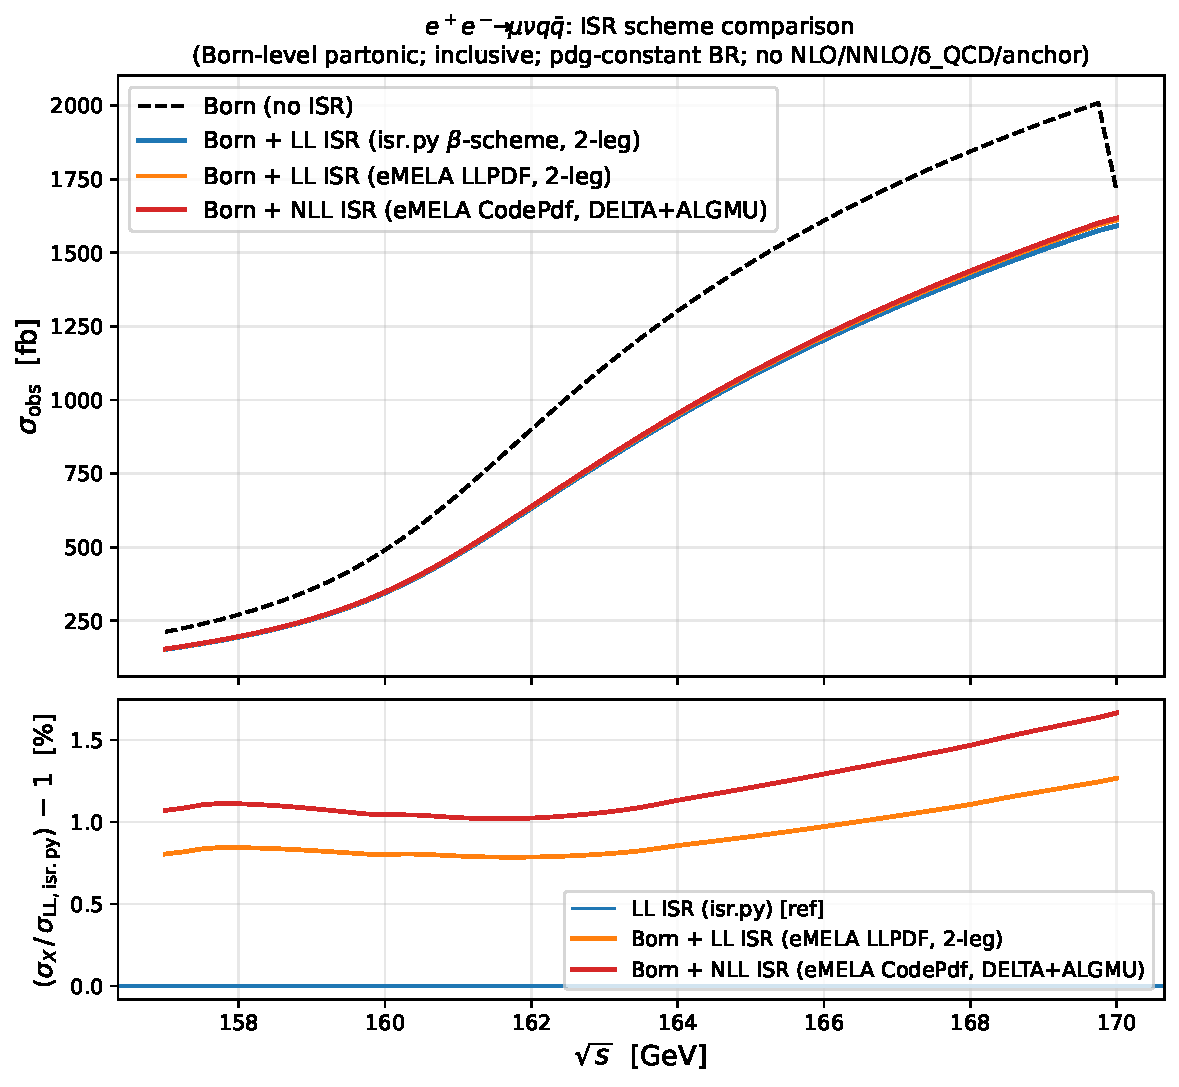
\includegraphics[width=0.49\linewidth]{figures/isr_comparison.pdf}
    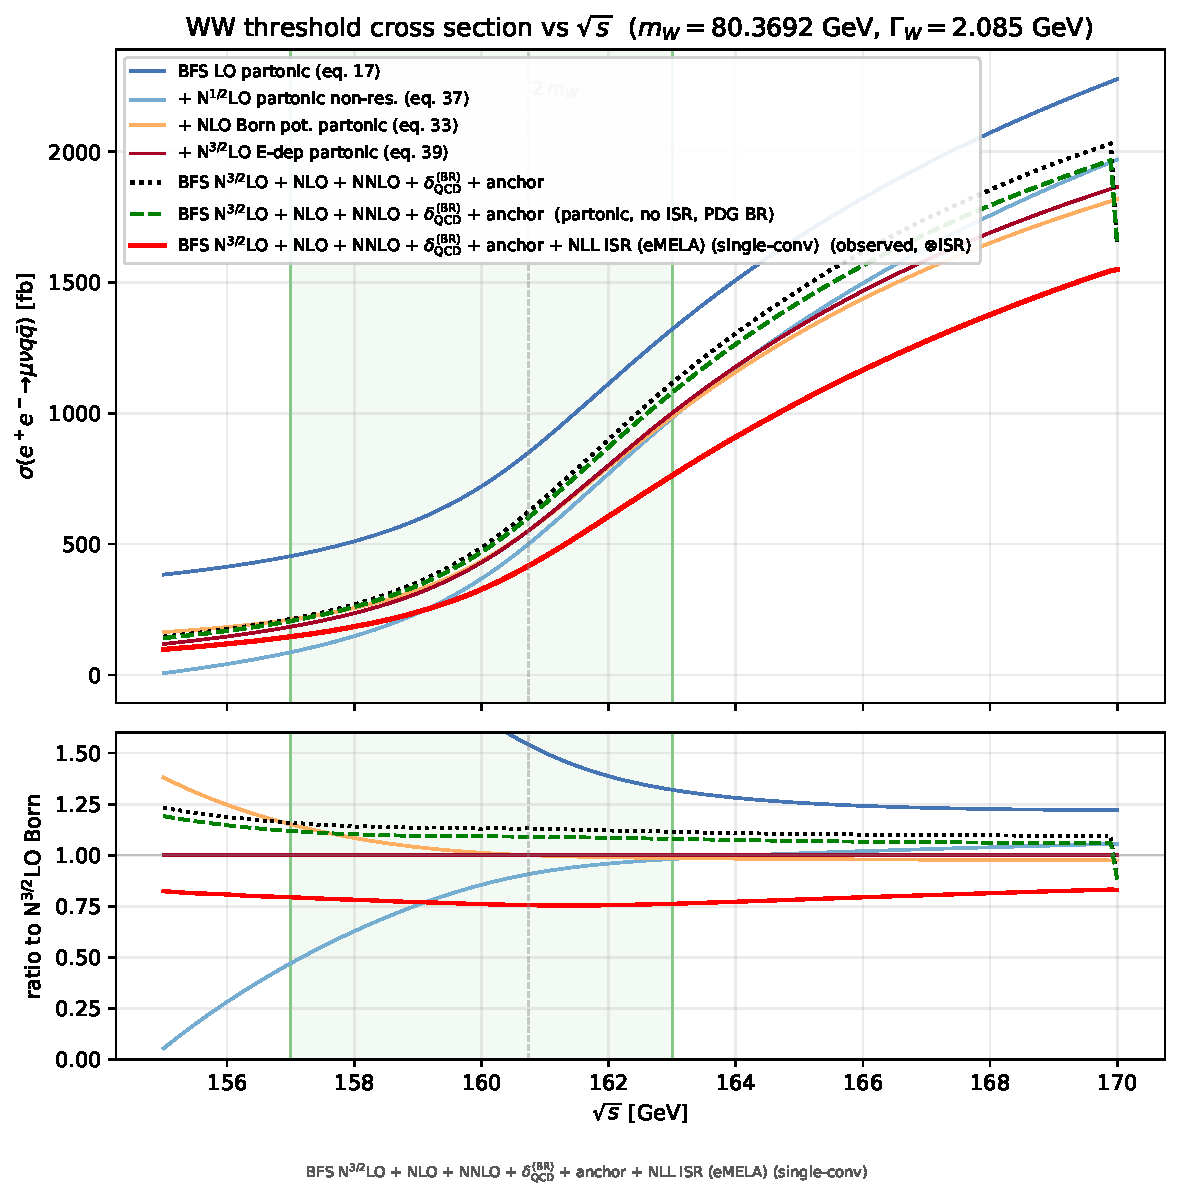
\includegraphics[width=0.49\linewidth]{figures/xsec_vs_sqrts.pdf}
    \caption{Left: effect of initial-state radiation (ISR) on the \WW
    production cross section near threshold, comparing the no-ISR result
    with the analytic LL$+$exp and the eMELA NLL convolutions.
    Right: predicted inclusive \WW production cross section as a function
    of the centre-of-mass energy, showing the build-up of the BFS chain
    (Born, NLO, NNLO, and the exact-Born anchor) with and without NLL
    ISR; the shaded band indicates the scan range
    $\sqrts\in[157,163]\GeV$ used in the fit. These plots are
    illustrative and will be replaced by publication-quality figures in a
    future version.}
    \label{fig:theory}
\end{figure}

The implementation has been validated against the reference tables of
Refs.~\cite{Beneke:2007zg,Actis:2008rb}. At the partonic level, the Born
and NLO results reproduce the BFS tables to four or five significant
digits across the scan window, and the dominant NNLO closed forms
reproduce the corresponding BFS NNLO table at the same level. The
anchoring to the exact \textsc{Whizard} four-fermion Born cross section
matches the BFS prescription to better than the per-mille level, and the
morphing used to interpolate the cross section in $(\mW,\GW,\sqrts)$ was
verified to be accurate at the few-ppm level, well below the statistical
sensitivity of the scan. A detailed account of these validations is
given in a separate technical note.


% =====================================================================
\section{Phenomenological analysis of the \boldmath \texorpdfstring{\WW}{W+W-} threshold scan}
\label{sec:scan}
% =====================================================================

The values of \mW and \GW are determined by fitting the predicted cross
section, as a function of \sqrts, to the measured \WW production rate. We
consider a baseline scan with seven equally-spaced points between
$\sqrts=157$ and $163\GeV$, with a spacing of $1\GeV$. We assume a total
integrated luminosity of $19.2\abinv$, corresponding to the FCC-ee
Feasibility Study baseline of a two-year run at the \WW threshold with
four interaction points~\cite{FCC:2025lpp}, split equally among the scan
points. The equal split is a simple, non-optimised choice; the results
scale with the assumed luminosity and its distribution among the scan
points. The measured cross sections are assumed to be obtained with a
signal selection efficiency of $0.8$, which inflates the statistical
uncertainties by $1/\sqrt{0.8}\approx 1.12$ with respect to the ideal
case.

The dependence of the predicted cross section on \mW, \GW, and \as is
shown in Figure~\ref{fig:variations} (left). As anticipated, a variation
of \mW mainly shifts the position of the threshold rise, while a
variation of \GW changes the steepness of the lineshape; the two
parameters therefore induce distinguishable shape distortions and can be
determined simultaneously, without assuming any relation between them.
The dependence on \as is small in the scan range. This makes it possible
to extract \mW and \GW from the threshold scan in a largely
model-independent way, enhancing the sensitivity to possible BSM
contributions to the W~width.

\begin{figure}[htbp]
    \centering
    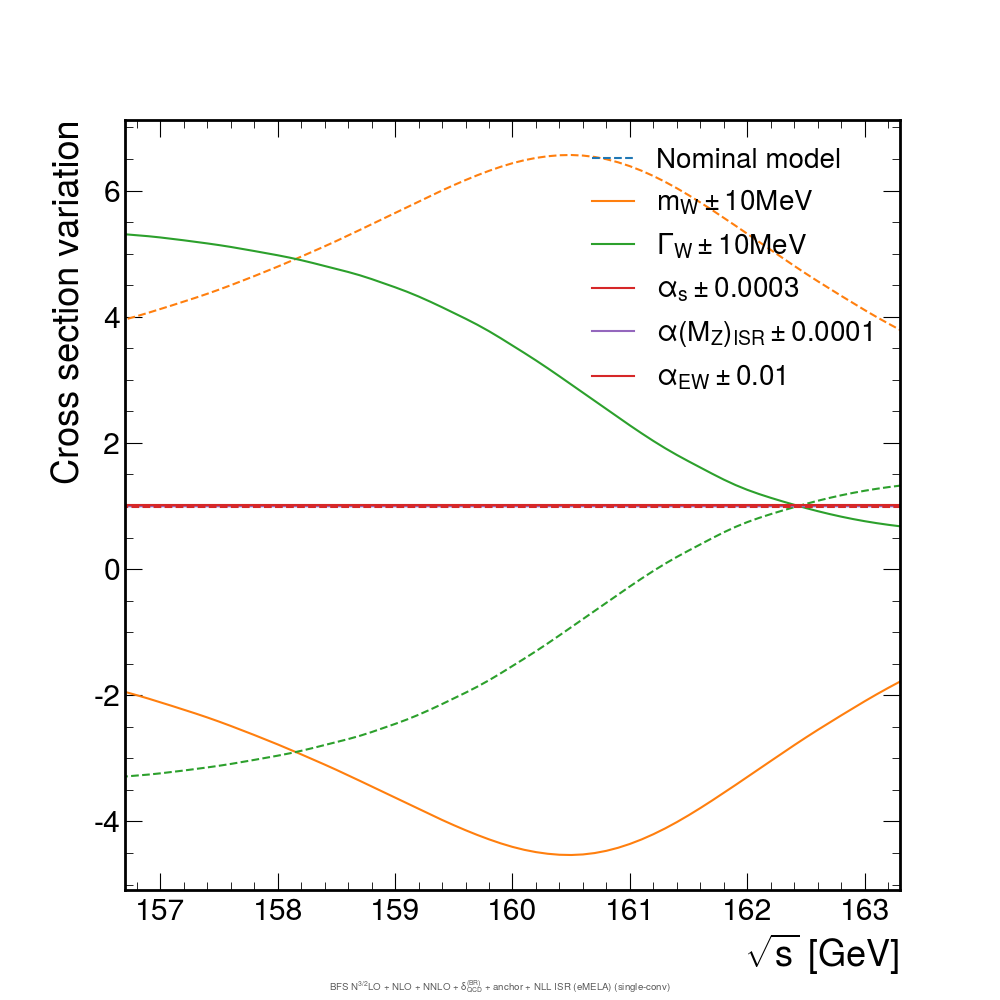
\includegraphics[width=0.49\linewidth]{figures/param_variations.png}
    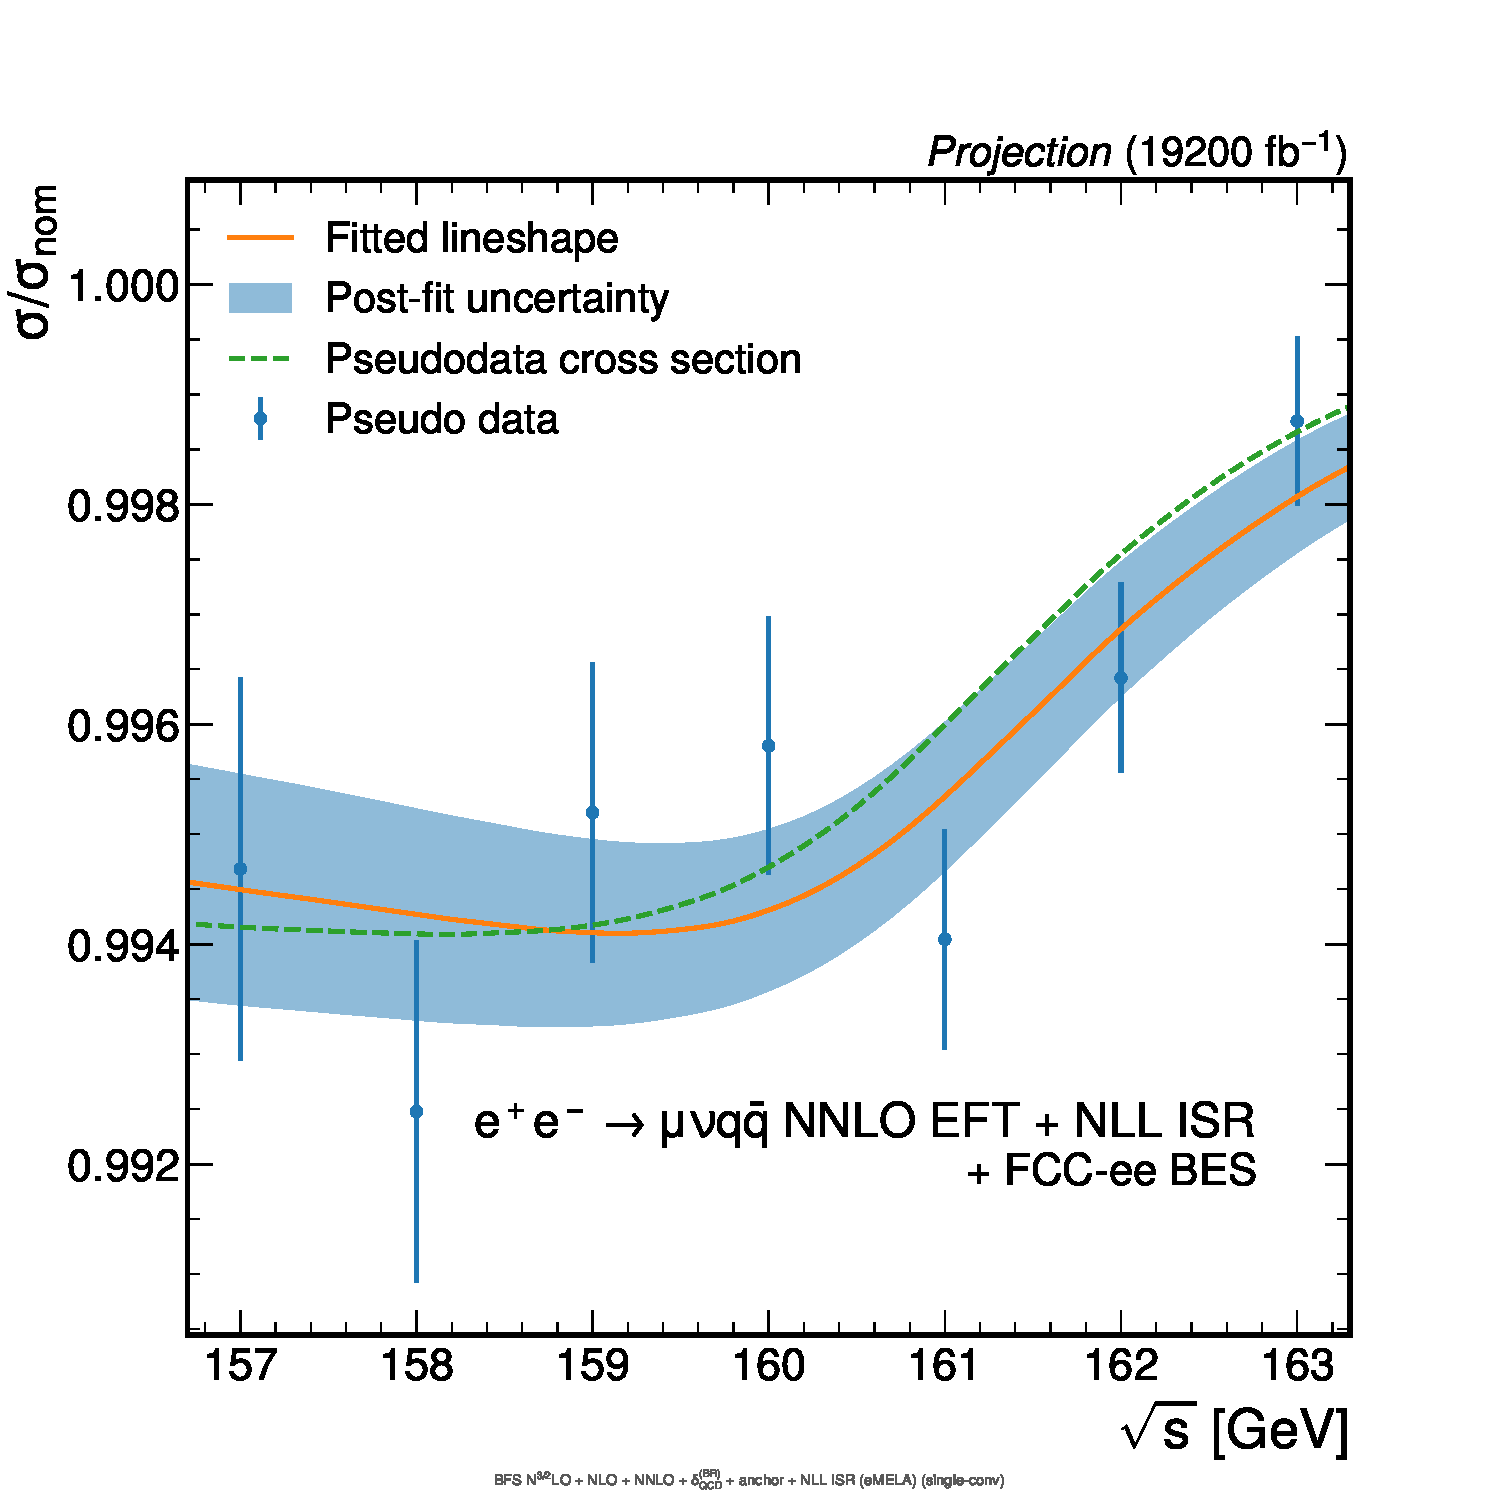
\includegraphics[width=0.49\linewidth]{figures/fit_scenario_ratio_pseudo.pdf}
    \caption{Left: dependence of the predicted \WW production cross
    section on \mW, \GW, and \as. The plot shows the ratio of the cross
    section after varying each parameter to the one obtained with the
    reference values. Right: fitted lineshape (solid line) as a function
    of the centre-of-mass energy, normalised to the reference cross
    section (horizontal dashed line). The fit is performed to pseudo-data
    (markers) generated with parameter values displaced from the
    reference. The uncertainty in the pseudo-data (vertical bars)
    represents the assumed experimental uncertainty in the \WW cross
    section, and the band corresponds to the post-fit uncertainty in the
    fitted cross section.}
    \label{fig:variations}
\end{figure}

The fit of the threshold lineshape is performed by minimising a \chisq
function in which the dependence of the predicted cross sections on \mW,
\GW, and \as, as well as on the beam energy calibration (BEC) and the
beam energy spread (BES), is incorporated through nuisance parameters.
The effect of these parameters is evaluated using discrete two-point
variations and interpolated, with an additional bilinear term that
captures the residual non-factorisable $(\mW,\GW)$ curvature. A
covariance matrix is built from the statistical uncertainty in the
measured cross sections and the uncertainty in the integrated
luminosity. For each scan point $i$, the statistical uncertainty in the
measured cross section ($\sigma_i$) is estimated as
$\sqrt{\sigma_i/\mathcal{L}_i}$, where $\mathcal{L}_i$ is the integrated
luminosity assigned to that point. The values of \mW and \GW are treated
as free-floating parameters, while the other parameters are constrained
with Gaussian priors representing external knowledge. Details on the
statistical model are given in Appendix~\ref{app:fit_model}.

In the fit, \asmz is constrained to an uncertainty of $10^{-4}$ according
to FCC-ee projections~\cite{dEnterria:2020cpv}. The value of
$\alpha(\mZ)$ entering the ISR is profiled with an uncertainty of
$4.7\times10^{-8}$, the FCC-ee Tera-Z projection~\cite{Riembau:2025xxx},
and the parametric dependence of the overall EW coupling normalisation is
profiled as a flat cross-section rescale with a prior of
$\delta\sigma/\sigma = 1.2\times 10^{-5} = 2\,\delta\alpha/\alpha$ from
the same projection; both are found to be negligible. The luminosity
uncertainty is taken from the projected precision of the di-photon
luminosity measurement~\cite{CarloniCalame:2019dyk}:
$2\times10^{-4}$ per-point uncorrelated, rescaled with the collected
luminosity at each point, and $1\times10^{-4}$ fully correlated. The
beam energy calibration uncertainty follows the FCC-ee
resonant-depolarisation projection~\cite{FCC:2025lpp,Blondel:2019jmp}:
$0.1\MeV$ point-to-point uncorrelated and $0.3\MeV$ fully correlated on
the collision energy. For the beam energy spread we assume a relative
knowledge of $1\%$ ($0.5\%$) for the uncorrelated (correlated)
component~\cite{Blondel:2019jmp}. Finally, to emulate experimental
systematic uncertainties in the cross-section determination in advance
of the detector-level study, we include two placeholder cross-section
uncertainties, each sized as $30\%$ of the per-point statistical
uncertainty: one fully correlated and one fully uncorrelated across the
scan points, added directly to the covariance matrix.
\TODO{the placeholder cross-section systematic uncertainties and the
BES knowledge components will be refined once the detector-level study
is available; the dependence of the results on all input uncertainties
is studied explicitly in Section~\ref{sec:param_scans}.}

Figure~\ref{fig:variations} (right) shows the fitted lineshape obtained
from a fit to pseudo-data generated with \mW and \GW displaced from the
reference values. Good closure is observed between the fitted and the
predicted cross section within the considered uncertainties, validating
the fit against arbitrary choices of \mW and \GW. The results presented
in the remainder of this section are instead obtained with an Asimov
data set~\cite{Cowan:2010js}, for which the pseudo-data correspond to the
central value of the prediction.


\begin{table}[htpb]
    \centering
\begin{tabular}{l|c|c|l}
Uncertainty source  & \mW [\MeV{}] & \GW [\MeV{}] & Input value \\ \hline
Experimental (stat.)              & 0.9 & 2.0 & $\mathcal{L} = 19.2\abinv$, $\varepsilon = 0.8$ \\
Parametric \mW                    & --  & 1.6 & free parameter \\
Parametric \GW                    & 0.8 & --  & free parameter \\
Parametric \as                    & 0.1 & 0.0 & $\delta\asmz = 10^{-4}$ \\
Parametric $\alpha(\mZ)_\mathrm{ISR}$ & 0.0 & 0.0 & $\delta\alpha = 4.7\times10^{-8}$ \\
Parametric EW normalisation       & 0.0 & 0.0 & $\delta\sigma/\sigma = 1.2\times10^{-5}$ \\ \hline
Luminosity calibration (uncorr.)  & 0.3 & 0.5 & $\delta L/L = 2\times10^{-4}$, per-point scaled \\
Luminosity calibration (corr.)    & 0.2 & 0.0 & $\delta L/L = 1\times10^{-4}$ \\
Beam energy calibration (uncorr.) & 0.0 & 0.1 & $\delta\sqrts = 0.1\MeV$ \\
Beam energy calibration (corr.)   & 0.2 & 0.0 & $\delta\sqrts = 0.3\MeV$ \\
Beam energy spread (uncorr.)      & 0.0 & 0.0 & $\delta\Delta E = 1\%$ \\
Beam energy spread (corr.)        & 0.0 & 0.0 & $\delta\Delta E = 0.5\%$ \\
Cross section (uncorr.)           & 0.4 & 0.8 & $30\%$ of stat.\ (placeholder) \\
Cross section (corr.)             & 0.5 & 0.5 & $30\%$ of stat.\ (placeholder) \\
\hline
Total experimental                & 1.5 & 2.9 & \\
Theory (ISR, NNLL truncation)     & 2.4 & 0.2 & unprofiled; $0.7$ shape-only (Section~\ref{sec:theory_unc}) \\
\end{tabular}
     \caption{Impact of the various sources of systematic uncertainty on
     the total uncertainty in \mW and \GW. The impacts are estimated as
     the difference in quadrature between the total uncertainty and an
     alternative fit in which the corresponding nuisance parameters are
     removed. The theoretical uncertainty is estimated separately, as
     described in Section~\ref{sec:theory_unc}. The cross-section
     systematic uncertainties are placeholder values in advance of the
     detector-level study, and additional experimental and machine-related
     systematic uncertainties are not yet included.}
     \label{tab:breakdown}
\end{table}


The results of the Asimov fit are summarised in
Table~\ref{tab:breakdown}. We find that \mW and \GW can be determined
with a total experimental precision of $1.5$ and $2.9\MeV$,
respectively, taking into account the experimental, parametric,
machine-related, and placeholder cross-section uncertainties considered
so far. The statistical
component alone amounts to $0.9$ and $2.0\MeV$ for \mW and \GW. With the
realistic di-photon luminosity and resonant-depolarisation
beam-calibration projections, the budget is statistics-dominated: the
leading systematic contributions to \mW are the placeholder
cross-section uncertainties, followed by the luminosity and the
correlated beam energy calibration, while the precision in \GW is driven
by the statistical uncertainty and by the parametric correlation with
\mW. A
correlation of $55\%$ between \mW and \GW is obtained from the fit, as
shown by the two-dimensional confidence intervals in
Figure~\ref{fig:contour}. We stress that the placeholder size of the
cross-section systematic uncertainties and the absence of detector-level
and additional machine-related systematic uncertainties imply that the
numbers in Table~\ref{tab:breakdown} are to be regarded as a preliminary
projection.

\begin{figure}[htpb]
    \centering
    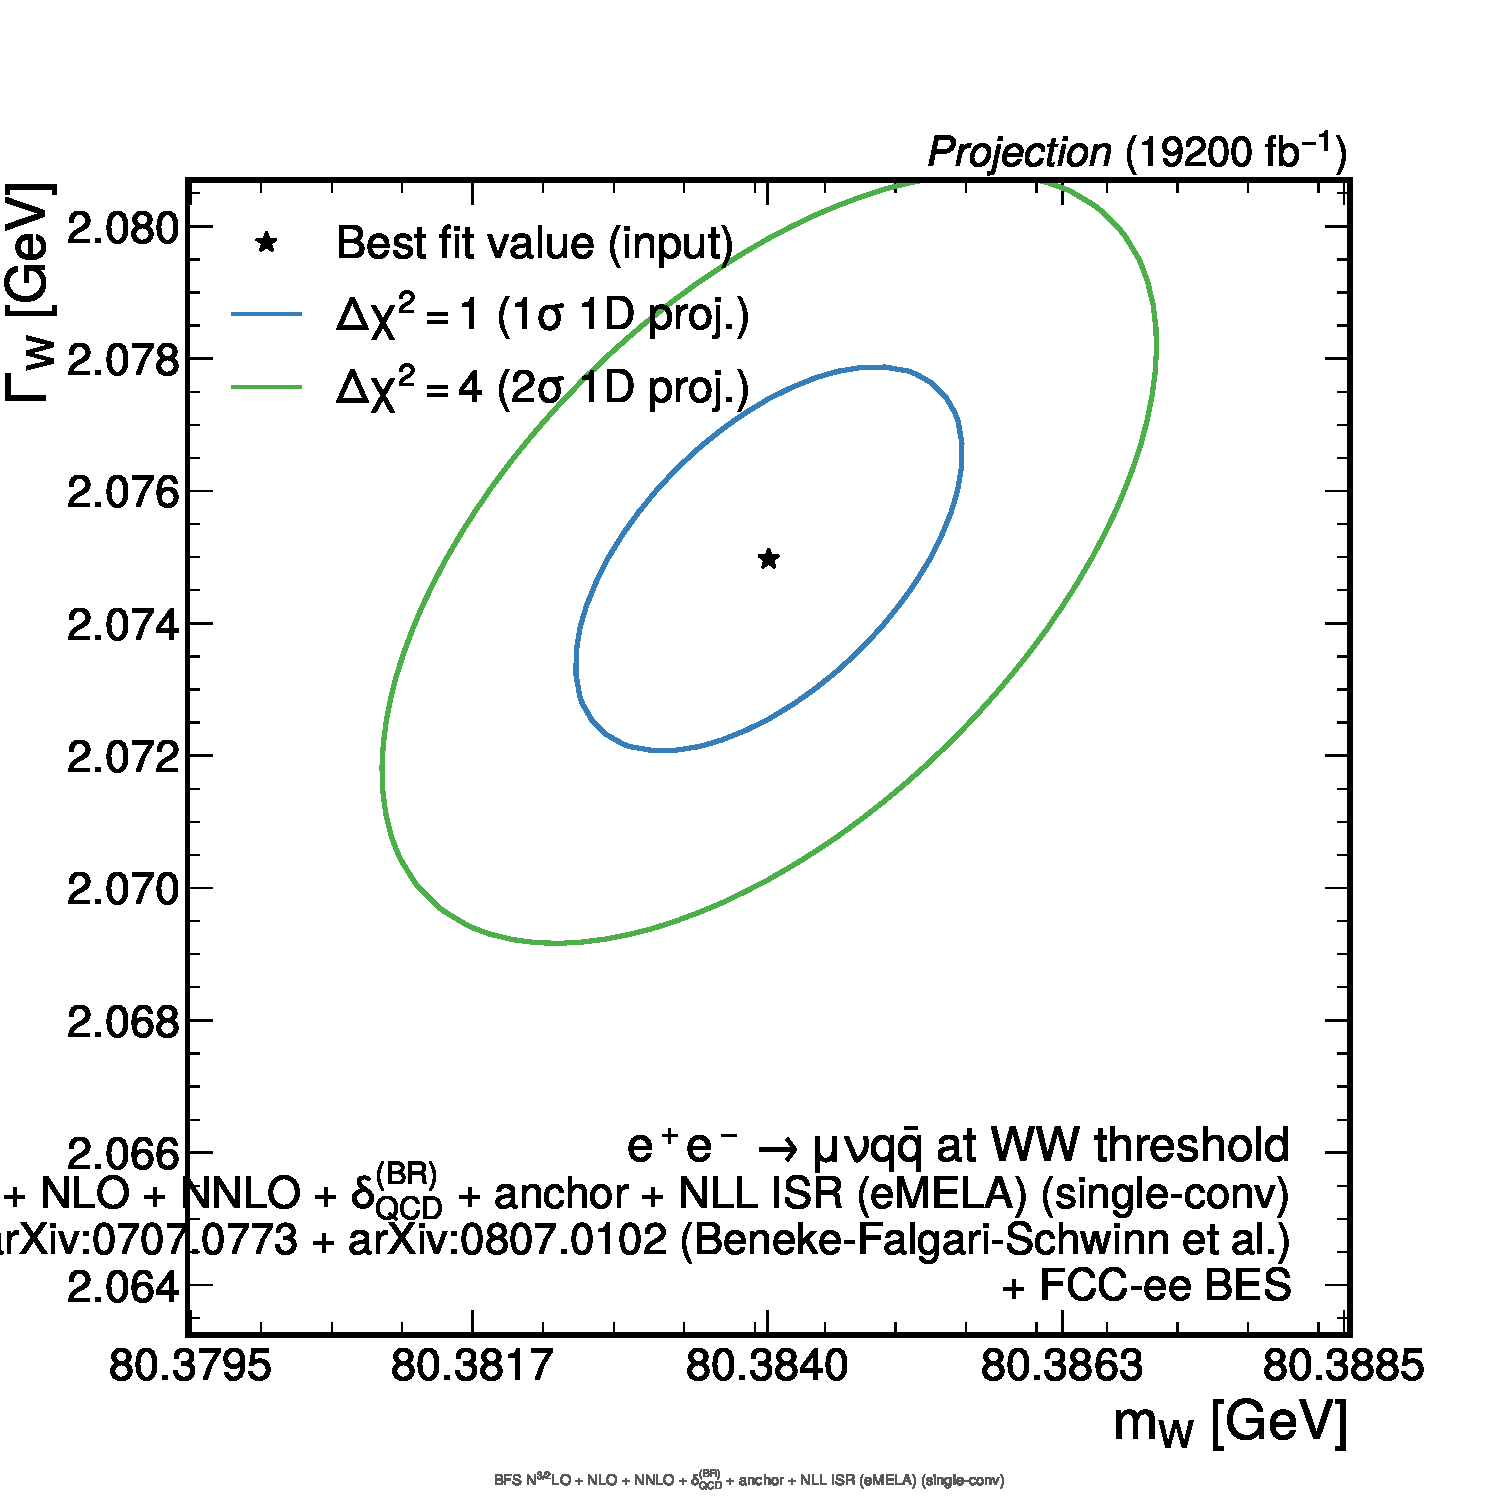
\includegraphics[width=0.55\linewidth]{figures/chi2_scan_mass_width.pdf}
    \caption{Two-dimensional confidence intervals in \mW and \GW,
    corresponding to the $68\%$ (inner ellipse) and $95\%$ (outer
    ellipse) confidence level, obtained from the Asimov fit of the \WW
    threshold scan.}
    \label{fig:contour}
\end{figure}


% =====================================================================
\section{Dependence of the results on the assumptions on systematic uncertainties}
\label{sec:param_scans}
% =====================================================================

The results of Section~\ref{sec:scan} rely on assumptions on the input
values for the various sources of systematic uncertainty, several of
which are still preliminary. It is therefore important to study the
dependence of the projected precision on these assumptions. To this end,
we present scans of the uncertainties in \mW and \GW as a function of the
input uncertainties for the profiled nuisance parameters, separately for
the point-to-point uncorrelated and correlated components where
relevant. With the results presented in this section, the numbers in
Table~\ref{tab:breakdown} can be rescaled to reflect any refinement in
the estimates of the input uncertainties.

The impact of the uncertainty in the integrated luminosity is shown in
Figure~\ref{fig:scan_lumi_alphas} (left). As expected, the luminosity
uncertainty has a larger impact on \mW than on \GW: an overall
normalisation uncertainty in the measured cross sections is partly
reabsorbed by a shift in the fitted threshold position, and therefore in
\mW, while it has a smaller effect on the shape that determines \GW. The
impact of the parametric uncertainty in \asmz is shown in
Figure~\ref{fig:scan_lumi_alphas} (right), and is found to be small for
both parameters over the considered range.

\begin{figure}[htpb]
    \centering
    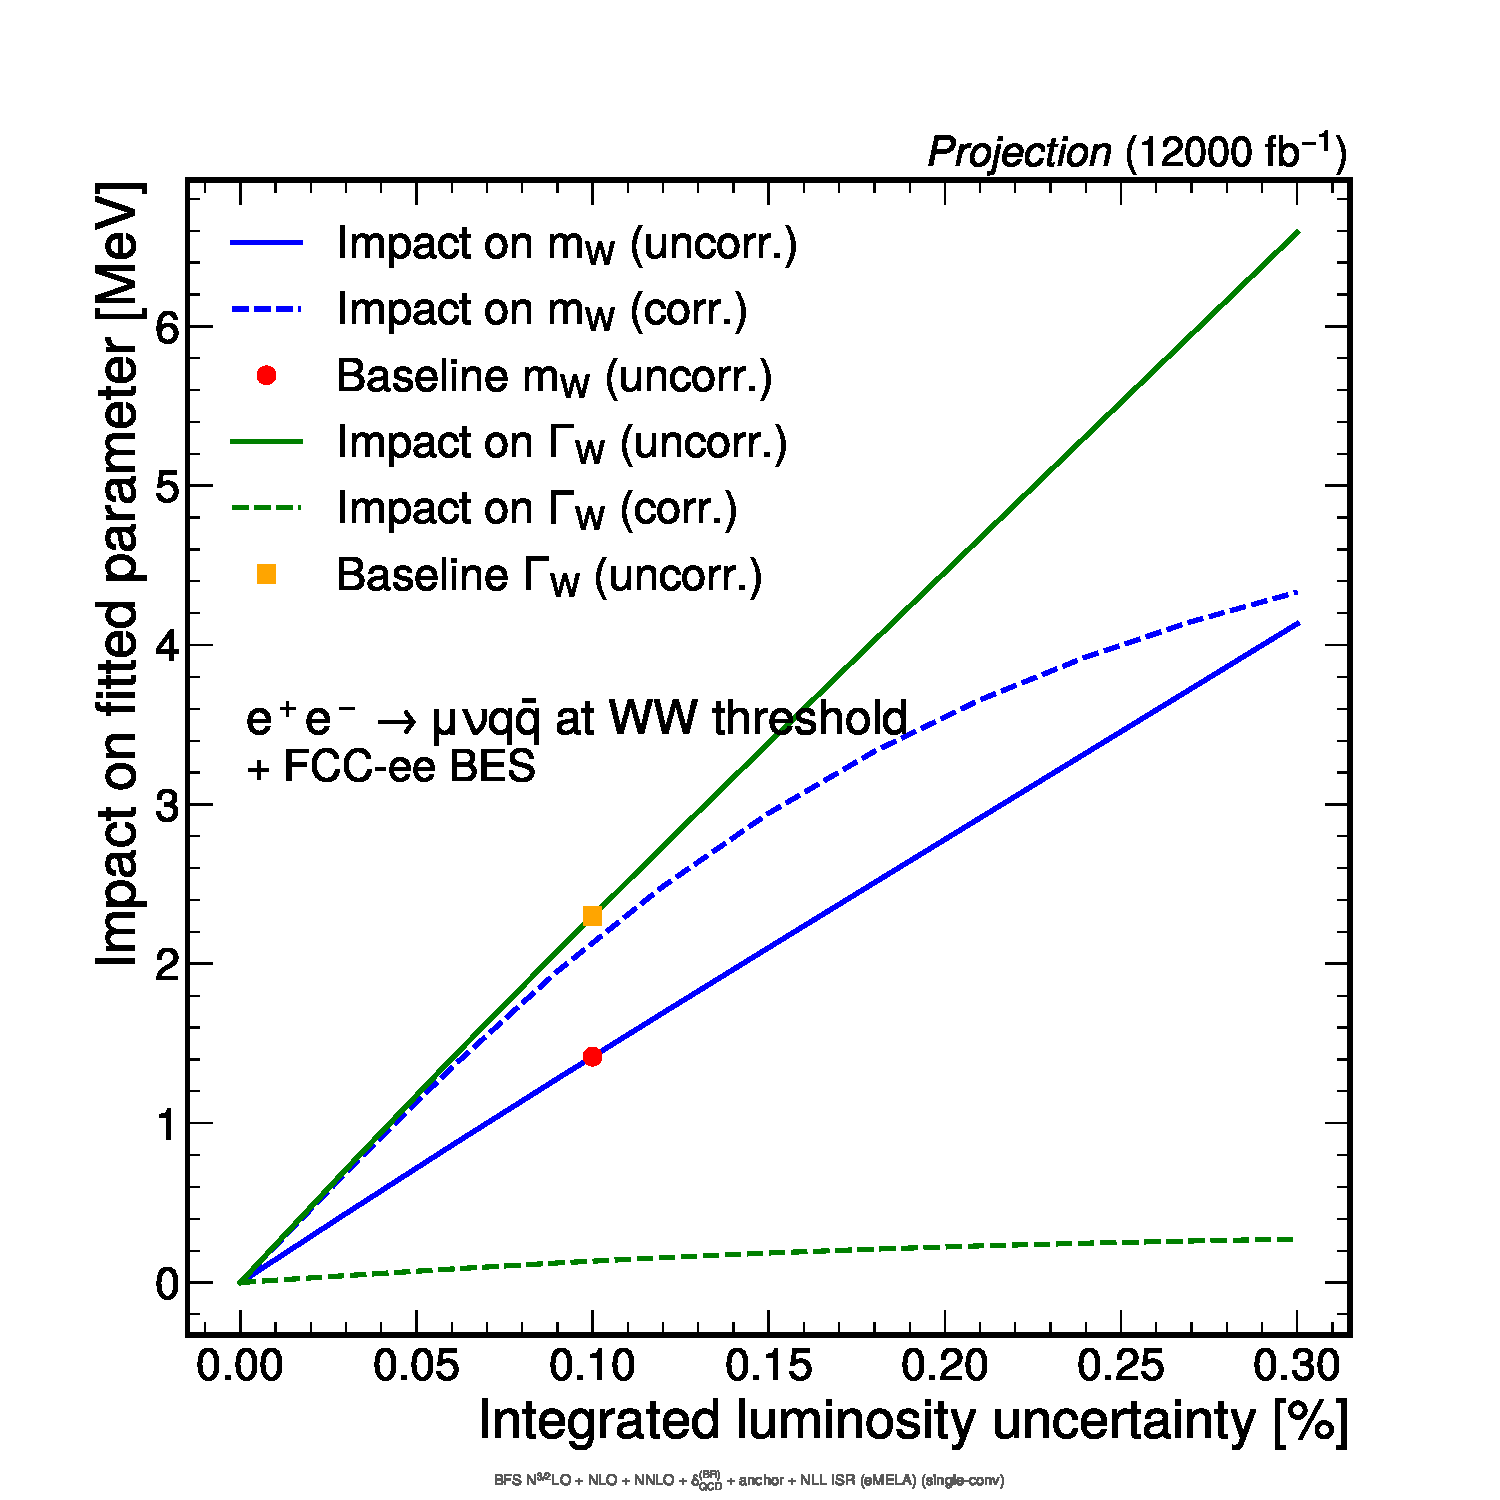
\includegraphics[width=0.49\linewidth]{figures/uncert_mass_width_vs_lumi.pdf}
    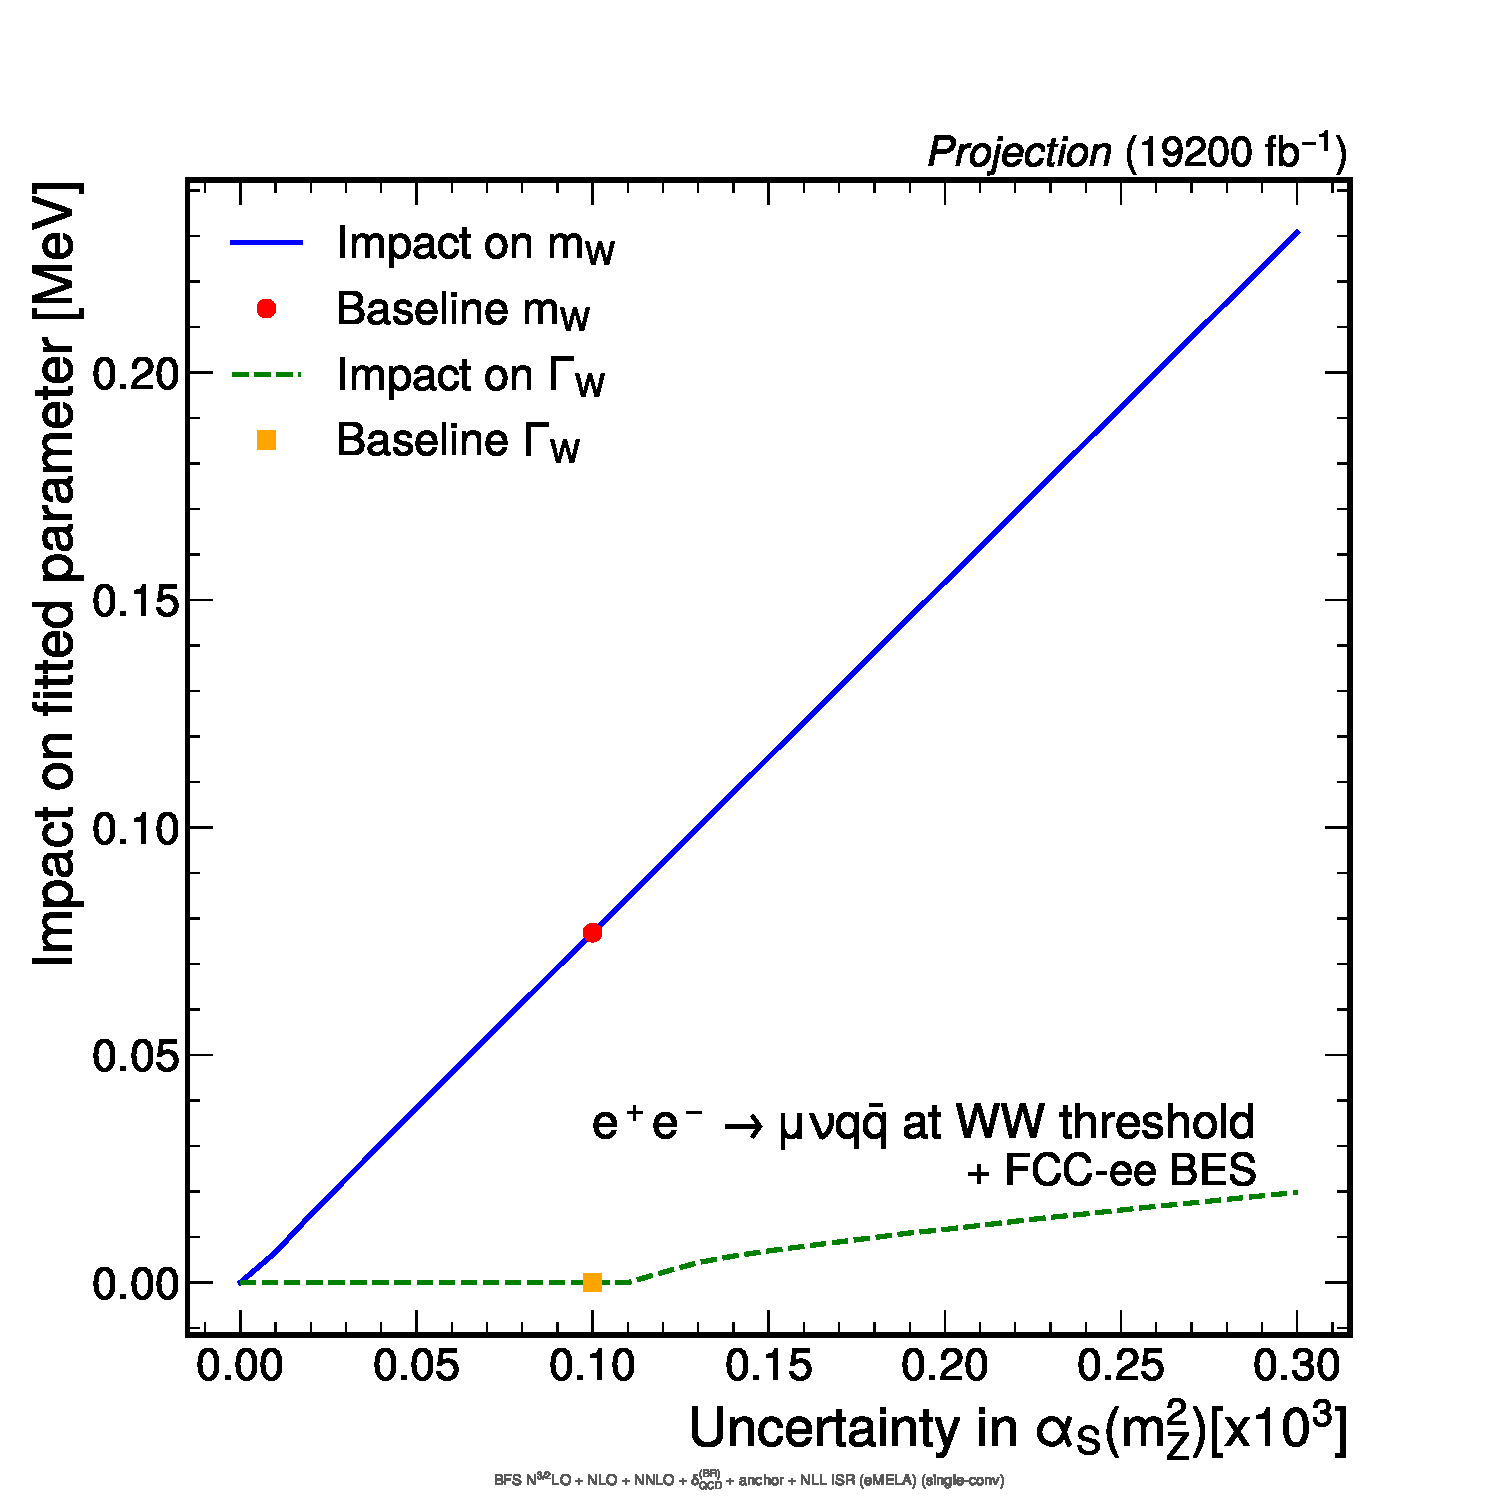
\includegraphics[width=0.49\linewidth]{figures/uncert_mass_width_vs_alphas.pdf}
    \caption{Impact on \mW (solid lines) and \GW (dashed lines) of the
    uncertainty in the integrated luminosity (left) and of the
    parametric uncertainty in \asmz (right). For the luminosity, the
    uncorrelated and correlated components are shown separately. The
    markers indicate the baseline assumptions used in
    Table~\ref{tab:breakdown}.}
    \label{fig:scan_lumi_alphas}
\end{figure}

The impact of the BEC and BES uncertainties is shown in
Figure~\ref{fig:scan_machine}. A correlated BEC uncertainty, which causes
an overall shift of the spectrum in \sqrts, translates directly into a
corresponding shift of the measured \mW by $\delta\sqrts/2$, as expected
from the fact that the threshold lies at $\sqrts\simeq 2\mW$; the same
shift has a much smaller effect on \GW, as it can be largely reabsorbed
by \mW. The BES uncertainty, on the other hand, has a stronger impact on
\GW than on \mW, since the beam energy spread smears the threshold rise
and is therefore partly degenerate with the width. These scans confirm
the importance of a precise calibration of the beam energy and of its
spread for the most precise determination of \mW and \GW.

\begin{figure}[htpb]
    \centering
    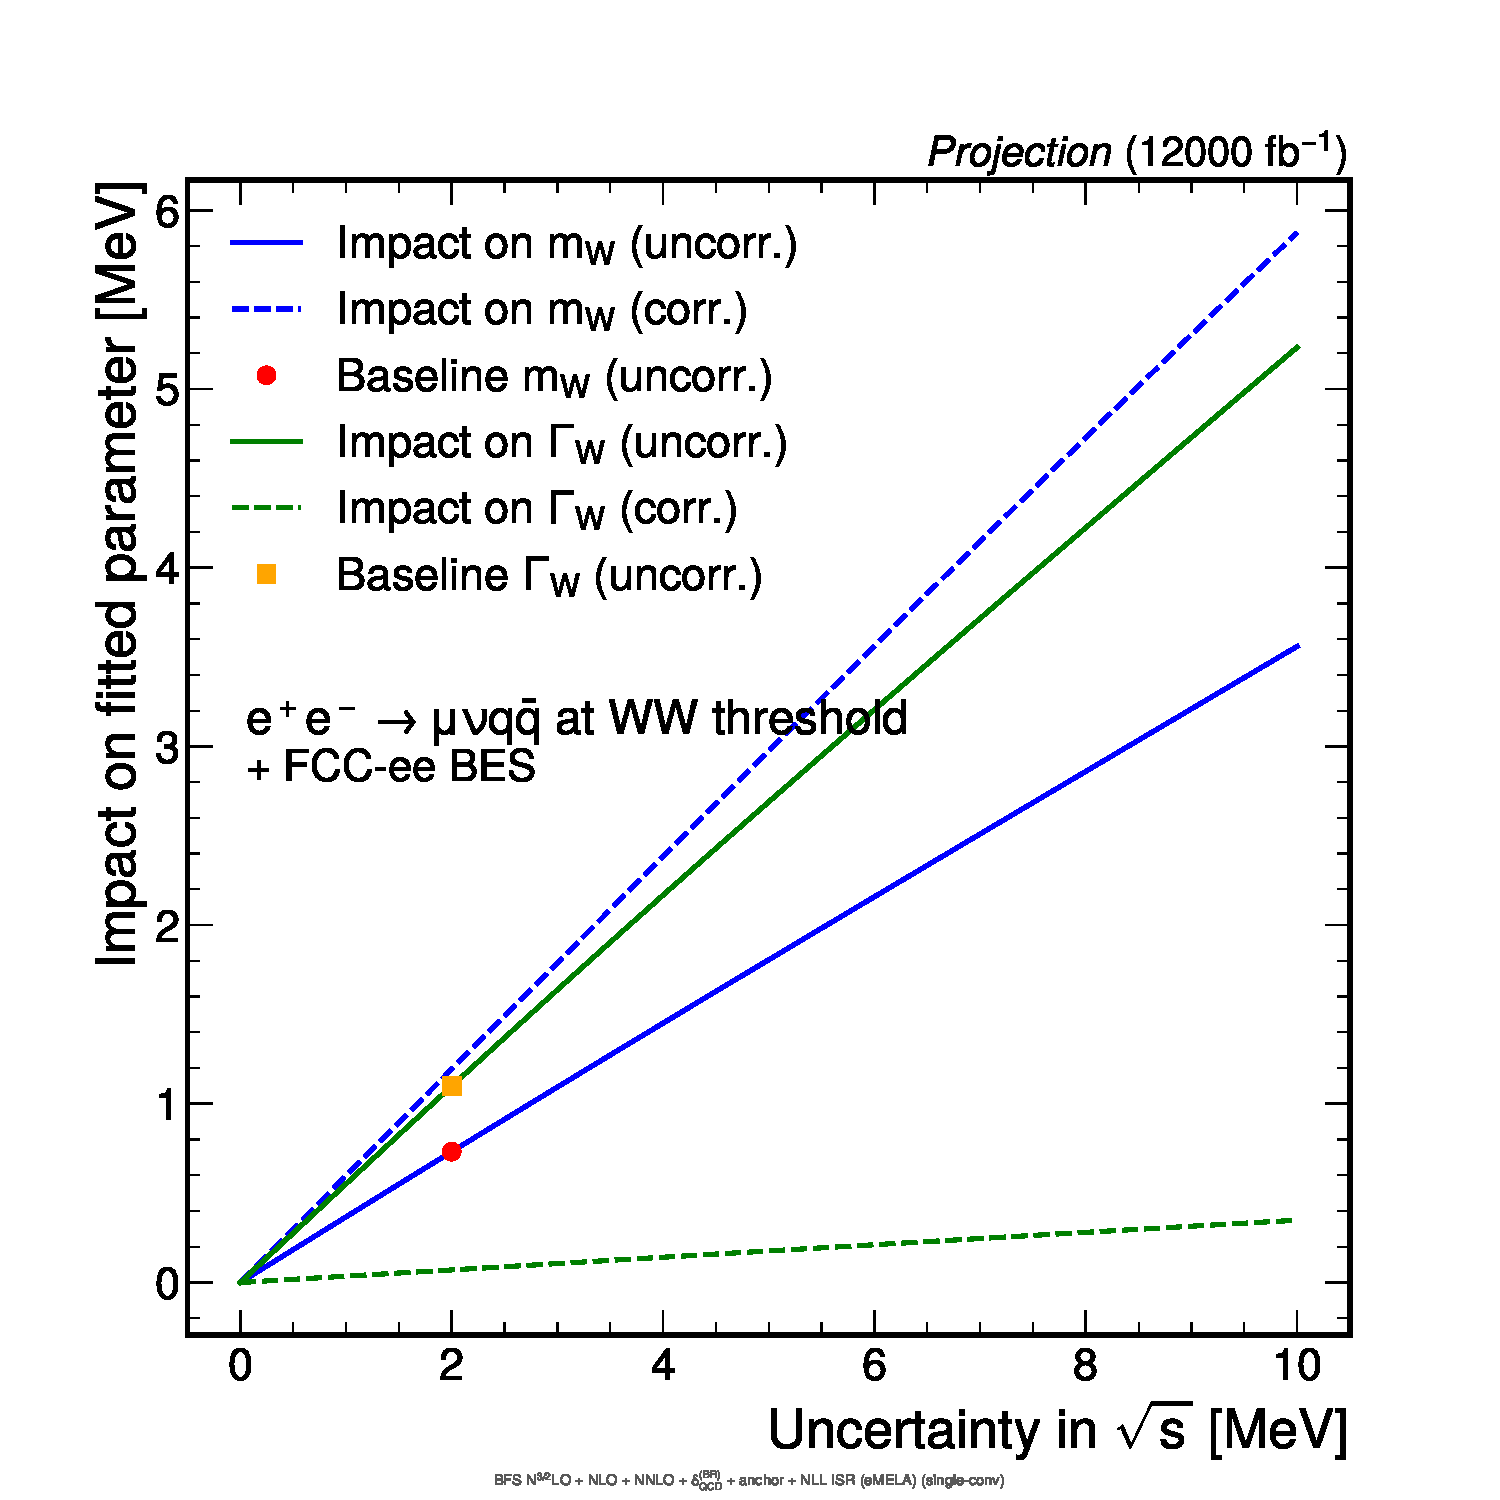
\includegraphics[width=0.49\linewidth]{figures/uncert_mass_width_vs_BEC.pdf}
    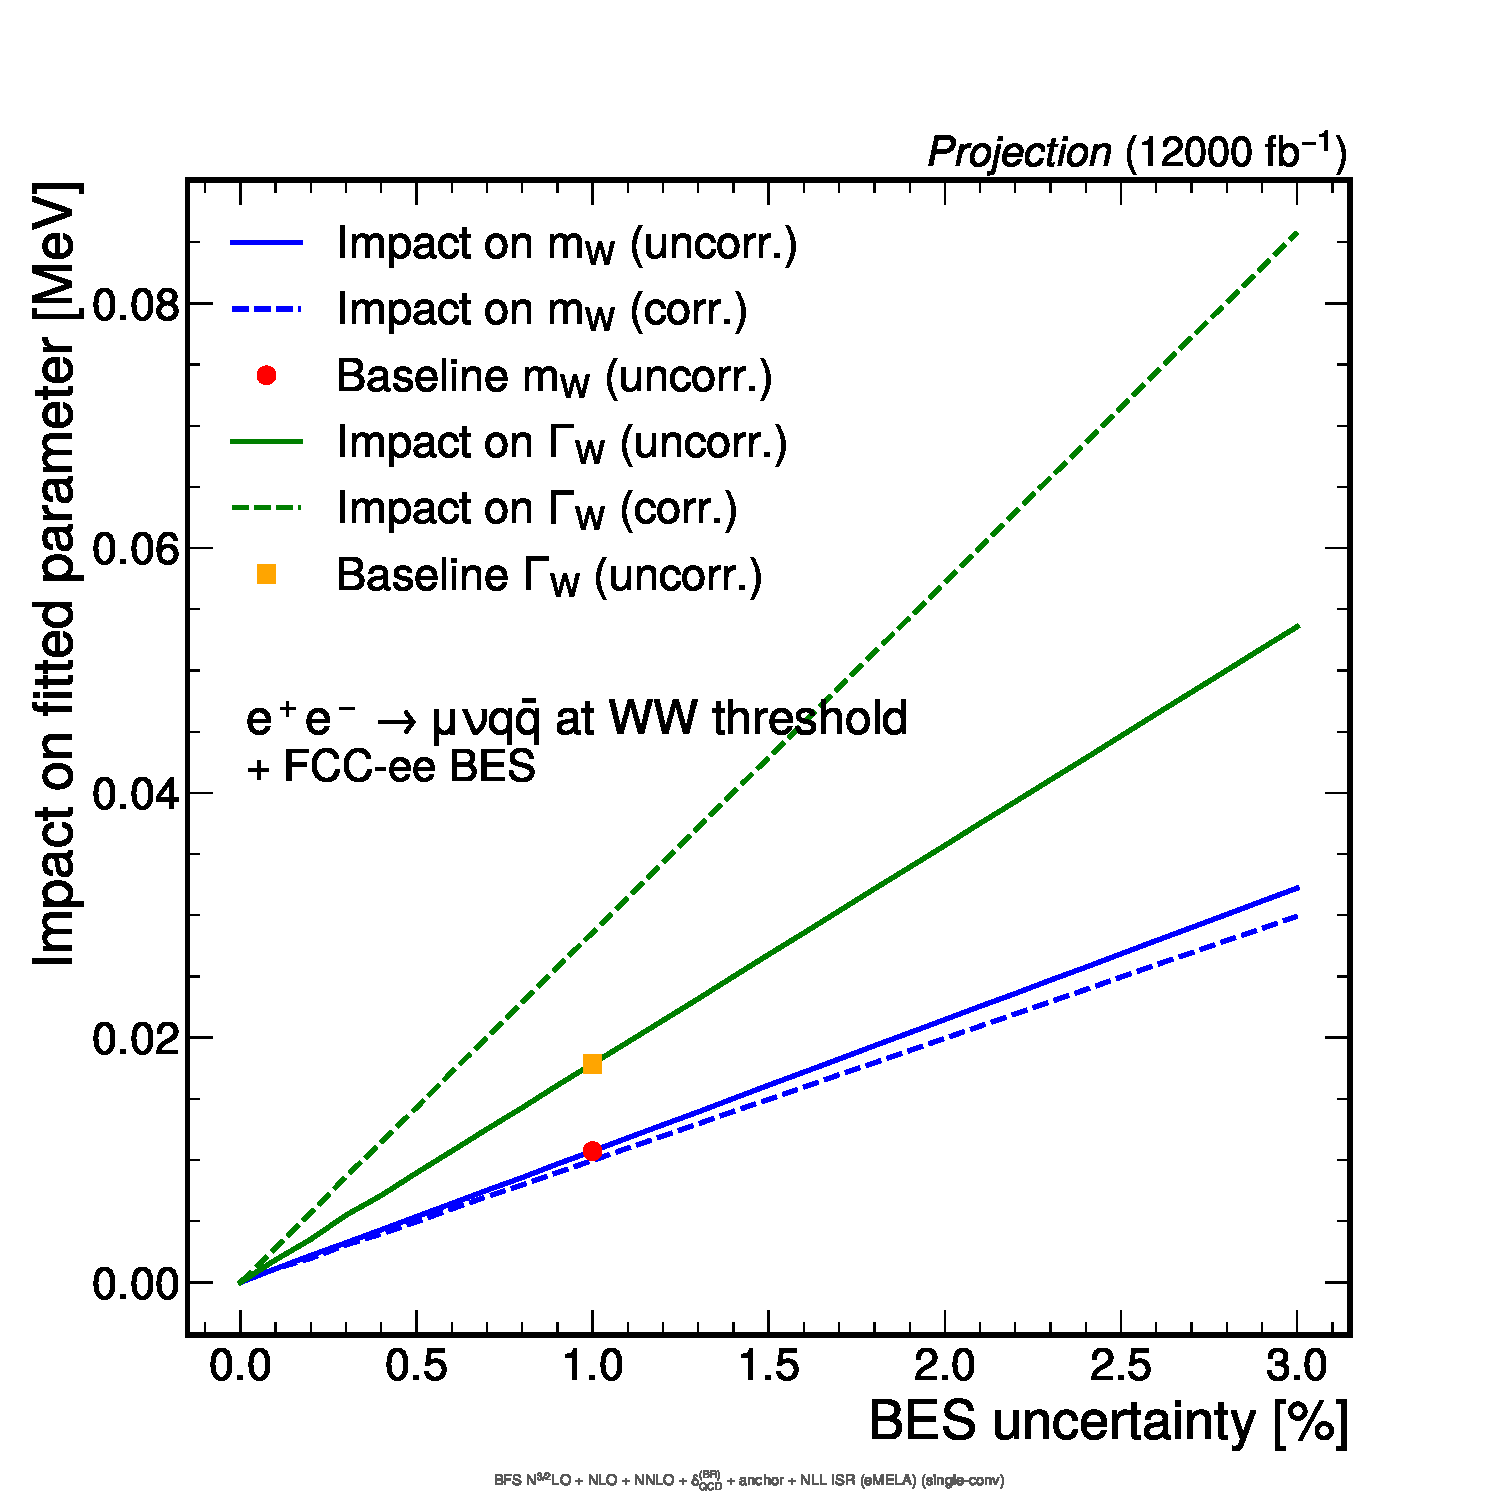
\includegraphics[width=0.49\linewidth]{figures/uncert_mass_width_vs_BES.pdf}
    \caption{Impact on \mW (solid lines) and \GW (dashed lines) of the
    uncertainties in the beam energy calibration (BEC, left) and beam
    energy spread (BES, right). The uncorrelated and correlated
    components are shown separately. The markers indicate the baseline
    assumptions used in Table~\ref{tab:breakdown}.}
    \label{fig:scan_machine}
\end{figure}


% =====================================================================
\section{Theoretical uncertainty from initial-state radiation}
\label{sec:theory_unc}
% =====================================================================

The dominant theoretical uncertainty in the determination of \mW from a
\WW threshold scan arises from the modelling of ISR. Because ISR shifts
the effective collision energy, an imperfect description of the photon
radiation directly biases the inferred threshold position and hence \mW.
We assess this uncertainty by exploiting the fact that our implementation
can convolute the partonic cross section with ISR at different orders of
accuracy.

We perform a cross-fit in which the pseudo-data are generated with the
baseline NLL ISR and the templates are built with the LL kernel
evaluated with the same $\alpha(\mZ)$, so that only the genuine NLL
terms differ, and read off the resulting bias in the fitted \mW. The
bias is $2.4\MeV$ with the baseline luminosity constraint, and reduces
to $0.7\MeV$ when the overall normalisation is left free in the fit.
The step from LL to NLL ISR is dominated by a change of the radiator
normalisation of about $0.3\%$, with only a sub-MeV distortion of the
lineshape: the larger figure therefore reflects the interplay of the
ISR normalisation with the luminosity constraint rather than a genuine
shape ambiguity. We conservatively take the pair ($2.4\MeV$ constrained,
$0.7\MeV$ shape-only) as the estimate of the NNLL-truncation uncertainty
on \mW, as reported in Table~\ref{tab:breakdown}. Replacing the NLL
description by the fully exponentiated analytic LL radiator instead
shifts \mW by about $18\MeV$ under the luminosity constraint --- again
almost entirely a normalisation effect ($0.8\MeV$ shape-only) ---
confirming that a NLL-accurate description of the ISR flux is required
at the FCC-ee precision. In addition, the uncertainty in the value of
$\alpha(\mZ)$ that enters the ISR, propagated as a profiled nuisance
parameter according to the FCC-ee Tera-Z
projection~\cite{Riembau:2025xxx}, is found to shift \mW by less than
$0.01\MeV$ and is therefore negligible. We also verified that the
template morphing closes at the few-ppm level under each ISR scheme, so
that no scheme-dependent re-derivation of the morphing is required.

This estimate covers only the ISR-related theoretical uncertainty.
A complete assessment of the theoretical uncertainty, including missing
higher-order EW corrections and the residual differences between the
EFT and the exact four-fermion calculation used for anchoring, is left
to future work. As in the case of the \ttbar threshold
scan~\cite{Defranchis:2025hfh}, improvements in the theoretical
predictions are expected to be a key ingredient in matching the
experimental precision achievable at FCC-ee.


% =====================================================================
\section{Summary and prospects}
\label{sec:summary}
% =====================================================================

We have presented a projection of the achievable precision in the
measurement of the W boson mass (\mW) and total width (\GW) from a
threshold scan at FCC-ee, in the centre-of-mass energy range
$\sqrts\in[157,163]\GeV$. The theoretical prediction of the \WW
production cross section was obtained from the BFS unstable-particle EFT,
implemented up to \NhalfLO in the EFT power counting and supplemented
with the dominant NNLO corrections, NLL initial-state radiation, and an
anchoring to the exact four-fermion Born cross section, and was validated
against the reference BFS calculations.

Using a maximum-likelihood fit of the predicted lineshape, with \mW and
\GW as free parameters, we project a statistical precision of about $0.9$
and $2.0\MeV$ on \mW and \GW, respectively, and a total experimental
precision of $1.5$ and $2.9\MeV$ including the leading parametric,
machine-related, and placeholder cross-section uncertainties considered
so far. We studied the
dependence of these results on the assumptions on the systematic
uncertainties, providing a means to rescale the projections as the input
estimates are refined, and we estimated the residual theoretical
uncertainty associated with the modelling of ISR to be $2.4\MeV$ on \mW
under the baseline luminosity constraint ($0.7\MeV$ from the lineshape
shape alone).

These results are preliminary in several respects. A detailed
detector-level study of the \WW cross section measurement, using
simulated events and including background processes and experimental
systematic uncertainties, is in preparation, following the strategy of
the companion \ttbar threshold study~\cite{Defranchis:2025hfh}.
Additional experimental and machine-related systematic uncertainties, as
well as a complete assessment of the theoretical uncertainty, remain to
be included; the cross-section systematic uncertainties are placeholder
values in advance of the detector-level study, and the equal luminosity
split among the scan points is a simple, non-optimised choice.
Nonetheless, the present study demonstrates
that a \WW threshold scan at FCC-ee has the potential to determine \mW
and \GW at the level of a few \MeV, providing a stringent test of the SM
through the comparison with the indirect determination from the EW fit,
and a direct, largely model-independent probe of possible BSM
contributions to the W~boson width.


\section*{Acknowledgements}
\TODO{acknowledgements to be added.}


\bibliographystyle{JHEP}
\bibliography{biblio}

\clearpage
\appendix

% =====================================================================
\section{Statistical model for the fit of the \boldmath \texorpdfstring{\WW}{W+W-} threshold scan}
\label{app:fit_model}
% =====================================================================

The \chisq function used for the analysis of the \WW threshold scan
depends on the parameters of interest (\mW and \GW), on the profiled SM
parameter \as, and on nuisance parameters that model the impact of the
systematic uncertainties ($\vec{\lambda}$). All systematic uncertainties
except the integrated luminosity are implemented as modifiers of the
predicted cross section. The \chisq function is defined as
\begin{align}
    \chisq(\mW,\GW,\as,\vec{\lambda}) =&~
    \vec{r}\,(\mW,\GW,\as,\vec{\lambda})^\mathrm{T}\,
    C_\mathrm{tot}^{-1}\,
    \vec{r}\,(\mW,\GW,\as,\vec{\lambda}) \nonumber \\
    &+ \left(\frac{\as-\as^0}{\delta\as}\right)^2 + \sum_i \lambda_i^2,
    \label{eq:chisq}
\end{align}
where
\begin{equation}
    \vec{r}\,(\mW,\GW,\as,\vec{\lambda}) =
    \vec{\sigma}_\mathrm{exp} -
    \vec{\sigma}_\mathrm{th}(\mW,\GW,\as,\vec{\lambda})
\end{equation}
are the residuals between the predicted and the (Asimov or pseudo-data)
measured cross sections. The penalty terms represent Gaussian
constraints on the nuisance parameters and on the parametric uncertainty
in \as, with $\as^0$ and $\delta\as$ the assumed central value and input
uncertainty for \as. The total covariance matrix is
\begin{equation}
    C_\mathrm{tot} = C_\mathrm{exp} + C_\mathrm{lumi}^\mathrm{uncorr} +
    C_\mathrm{lumi}^\mathrm{corr} + C_{\sigma}^\mathrm{uncorr} +
    C_{\sigma}^\mathrm{corr},
\end{equation}
where $C_\mathrm{exp}$ is the diagonal covariance matrix of the measured
cross sections, with
$[C_\mathrm{exp}]_{ij} =
\delta_{ij}\,\sigma_\mathrm{exp}^i/(\varepsilon\,\mathcal{L}_i)$ and
$\varepsilon$ the signal selection efficiency,
$C_\mathrm{lumi}^\mathrm{uncorr}$ and $C_\mathrm{lumi}^\mathrm{corr}$
are the uncorrelated and correlated components of the luminosity
uncertainty, and $C_{\sigma}^\mathrm{uncorr}$ and
$C_{\sigma}^\mathrm{corr}$ are the placeholder cross-section systematic
uncertainties, each sized as $30\%$ of the per-point statistical
uncertainty and taken fully uncorrelated (diagonal) and fully correlated
(rank-one), respectively. The profiled ISR coupling $\alpha(\mZ)$ and
the flat EW-normalisation nuisance carry Gaussian penalty terms
analogous to that of \as.

The dependence of the predicted cross section on each parameter is
modelled via an interpolation of two-point variations. We define the
nuisance parameters so that $\lambda_i=0$ corresponds to the baseline
value and $\lambda_i=1$ to a one-standard-deviation variation, so that
the cross section for arbitrary $\lambda_i$ is approximated by
\begin{equation}
    \vec{\sigma}_\mathrm{th}(\lambda_i) =
    \vec{\sigma}_\mathrm{th}(\lambda_i=0)
    \left\{1 + \lambda_i\left[
    \frac{\vec{\sigma}_\mathrm{th}(\lambda_i=1)}
         {\vec{\sigma}_\mathrm{th}(\lambda_i=0)} - 1 \right]\right\},
\end{equation}
and the joint dependence is obtained as the product of the individual
factors. For the parameters of interest \mW and \GW, the same procedure
is applied, with an additional bilinear term
\begin{equation}
    x_{ab}(\sqrts) =
    \frac{1+m_\mathrm{corner}(\sqrts)}
         {(1+m_a(\sqrts))(1+m_b(\sqrts))} - 1,
    \qquad a=\mW,\; b=\GW,
\end{equation}
built from a corner template in which both parameters are displaced
simultaneously. This captures the residual non-factorisable $(\mW,\GW)$
curvature that the product of per-parameter factors misses, and was
verified to reduce the corresponding closure bias on \mW to the
$\mathcal{O}(\keV)$ level. The \chisq function is minimised with the
\textsc{iminuit} package~\cite{iminuit} to obtain the best-fit values
and the covariance matrix. The parameter scans of
Section~\ref{sec:param_scans} are obtained by rescaling the
corresponding penalty terms and covariance components.


\end{document}
